

\chapter{Entropy and information theory}

\section{Entropy and its basic properties}
In this chapter we give an introduction to
$\textbf{information theory}$, a beautiful theory at
the intersection of ergodic theory, probability,
statistics, computer science, and branches of
engineering and physics.

Throughout the chapter, $X_1,X_2,X_3,\ldots$ will
denote a stationary ergodic sequence of random
variables taking values in a finite set
$A=\{\alpha_1,\ldots,\alpha_d \}$. We think of the
sequence as an $\textbf{information source}$,
emitting successive symbols from the set $A$, which
in this context will be referred to as the
$\textbf{alphabet}$. Think of a long text in English
or some other language\footnote{It may seem unusual to you that language is
considered as a statistical source, but spoken and
written language does exhibit very clear statistical
characteristics. Note that information theory makes no
attempt to address the \emph{meaning} (or usefulness) of a
string of text. Thus, the word ``information'' is used
in a slightly different meaning in information theory
versus how an ordinary person might use it. For
example, a string of random unbiased binary bits might
appear to contain very little information to a
layperson, but in the information theory sense this
kind of string has the highest possible information
content for a binary string of given length.}; a sequence of
bits being transmitted from one computer to another
over a network; data sampled by a scientific
instrument over time, etc.\ --- all of these are
examples of information sources which in suitable
circumstances are well-modeled by a stationary ergodic
sequence over a finite alphabet.

A fundamental problem of information theory is to
measure the information content of the source. This is
a numerical quantity which has come to be known as
$\textbf{entropy}$. We will define it and also try to
explain what the number it gives means. E.g., if the
entropy of a source is $3.5$, what does that tell us
regarding the difficulty of storing or communicating
information coming from the source?

Let us start with the simplest case of an i.i.d.\
sequence. Denote $p_k = \mathrm{P}(X_1 = \alpha_k)$.
The probability vector $(p_1,\ldots,p_d)$ gives the
relative frequencies of occurrence of each of the
symbols $\alpha_1,\ldots,\alpha_d$, and for an
i.i.d.\ sequence completely characterizes the
statistical properties of the sequence, so entropy
will simply be a function of the numbers
$p_1,\ldots,p_d$. We define it as

\[
H(p_1,\ldots,p_d) = -\sum_{k=1}^d p_k \log_2(p_k),
\]

\noindent with the convention that $0\log 0 = 0$. The logarithm
is traditionally taken to base $2$, to reflect the
importance of entropy in computer science and
engineering, although in certain fields (notably
thermodynamics and statistical physics) the natural
base is used, and any other base may be used as long
as it is used consistently in all formulas. If the
base $2$ is used, we say that entropy is measured in
units of $\textbf{bits}$. The letter $H$ used for the
entropy function is actually a capital Greek \emph{eta},
the first letter of the Greek word
\emph{entropia}\footnote{See the Wikipedia article
\href{http://en.wikipedia.org/wiki/History_of_entropy\#Information_theory}{http://en.wikipedia.org/wiki/History\emph{of}entropy\#Information\_theory}
for an amusing and often-told story about the origin
of the term entropy in information theory.}.

Note that entropy can be regarded as the average of
the quantity $-\log_2 p_k$ weighted by the
probabilities $p_k$. Thus, sometimes we write

\[
H(p_1,\ldots,p_k) = -\mathbf{E} \log_2 p(X),
\]

\noindent where $X$ is a random variable representing a source
symbol (i.e., $\mathrm{P}(X=\alpha_k)=p_k$ for each
$1\le k\le d$, and $p(\alpha_k)=p_k$ represents the
probability of each symbol. (It is a distinctive and
somewhat curious feature of information theory that
probabilities are often themselves regarded as random
variables.)

\begin{example}
In the case of a $2$-symbol alphabet ($d=2$), the
entropy function is usually written simply as a
function of one variable, i.e.,

\[
H(p) = -p\log_2 p - (1-p) \log_2 (1-p)
\]

\noindent This function is concave, has the symmetry
$H(p)=H(1-p)$, equal to $0$ at $p=0$ and $p=1$, and
takes the maximum value $H(1/2)=1$ at $p=1/2$ (see
Figure 6).
\end{example}

\begin{center}
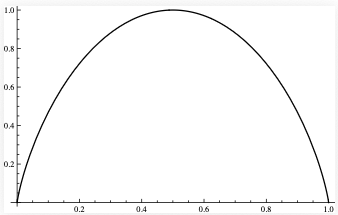
\includegraphics[width=0.55\linewidth]{figures/entropy.png}\\[0.6em]
{\small Figure 6: The entropy function $H(p)$ for a two-value
distribution}
\end{center}

\begin{lem}[Gibbs's inequality]
If $(p_1,\ldots,p_d)$ is a probability vector and
$(q_1,\ldots,q_d)$ is a \emph{sub-probability} vector,
i.e., we have $p_k,q_k\ge 0$, $\sum_k p_k = 1$ and
$\sum q_k \le 1$, then

\[
-\sum_{k=1}^d p_i \log p_i \le -\sum_{k=1}^d p_i \log q_i,
\]

\noindent with equality holding if and only the two vectors are
equal.
\end{lem}

\begin{proof}
The form of the inequality is unchanged by changing
the logarithm basis, so we use the natural logarithm.
Since $\log x \le x-1$ for all $x>0$, we have

\begin{align*}
-\sum_{k=1}^d p_k (\log q_k-\log p_k) &=
-\sum_{k=1}^d p_k \log\left( \frac{q_k}{p_k}\right)
\ge -\sum_{k=1}^d p_k \left( \frac{q_k}{p_k}-1 \right) \\ &= -\sum_k q_k + \sum_k p_k \ge -1+1 = 0.
\end{align*}

\end{proof}

\begin{lem}[Properties of the entropy function]
\label{lem-entropy-properties}
The entropy function of $d$-dimensional probability
vectors $(p_1,\ldots,p_d)$ satisfies:

\begin{enumerate}[label=\arabic*.]
\item $0 \le H(p_1,\ldots,p_d) \le \log_2 d$

\item $H(p_1,\ldots,p_d)=0$ if and only if $p_k=1$ for some
$k$ (and all the other $p_j$'s are 0).

\item $H(p_1,\ldots,p_d)=\log_2 d$ if and only if $p_k=1/d$
for all $k$.

\item $H(\mathbf{p}\otimes \mathbf{q}) = H(\mathbf{p}) +
H(\mathbf{q})$,
where if $\mathbf{p}=(p_1,\ldots,p_d)$ and
$\mathbf{q}=(q_1,\ldots,q_\ell)$, we use the notation
$\mathbf{p}\otimes\mathbf{q}$ to denote the
probability vector $(p_i q_j)_{i,j}$ on the product
of two alphabets of sizes $d$ and $\ell$.

\item $H(p_1,\ldots,p_d)$ is a concave function.
\end{enumerate}

\end{lem}

\begin{xexercise}
Prove Lemma \ref{lem-entropy-properties}.
\end{xexercise}

\section{The noiseless coding theorem}
Our first interpretation of the entropy function will
be in terms of the problem of
$\textbf{noiseless coding}$. Recall that the
information source emits symbols in the finite
alphabet $A=\{\alpha_1,\ldots,\alpha_d\}$. To
transmit the symbol over a digital communication
channel or store it on a computer storage system
(which is the same as transmission, except we're
transmitting it to ourselves in the future rather than
to a different physical location), we need to encode
the symbols as binary bits. We assume that the storage
system or communication system are
$\textbf{noiseless}$, i.e., no corruption of our data
is expected to occur.

What is a good way to encode the symbols as binary
bits? A naive approach would be to allocate $d$
distinct binary strings, one for each of the symbols.
Since the strings need to be distinct so that the
transmission can be decoded on the other end,
obviously it is necessary (and sufficient) for the
strings to be of length $\lceil \log_2 d\rceil$.
Thus, in terms of efficiency, this method uses the
channel approximately $\log_2 d$ times for every
symbol encoded.

But perhaps we can do better? For example, it is
possible that some of the symbols occur more
frequently than others. A more sophisticated approach
would be to assign binary strings of \emph{different}
lengths to the different symbols, assigning the
shorter strings to more frequently occurring symbols.
One must be careful however to make sure that the
transmission, which may consist of the concatenation
of several of the strings used to encode a succession
of source symbols, can be faithfully recovered. This
leads to the idea of $\textbf{codes}$.

\begin{defn}
Let $\{0,1\}^*=\cup_{n=1}^\infty \{0,1\}^n$ be the
set of all finite binary sequences (which we will call
$\textbf{words}$ or $\textbf{strings}$). A
$\textbf{code}$ for the alphabet
$A=\{ \alpha_1,\ldots,\alpha_d\}$ is a collection
$(w_k)_{k=1}^d$ of words in $\{0,1\}^*$. We say the
code is $\textbf{uniquely decodable}$ if any word
formed as a concatenation
$w_{j_1}w_{j_2}\ldots w_{j_m}$ of words in the code
can be decoded in a unique way, i.e., it is not equal
to any other concatenation of words from the same
code. We say that the code is a $\textbf{prefix code}$
if no word $w_i$ in the code is a prefix of another
word $w_j$.
\end{defn}

\noindent It is obvious that any prefix code is uniquely
decodable, since, when reading a concatenation of
words, we know immediately when a word terminates and
the next word begins. Not all uniquely decodable codes
are prefix codes, however (the code $0, 01, 011$ is
an example). It is however true that uniquely
decodable codes that are not prefix codes are in some
sense pointless and for all practical purposes they
may be ignored --- see Exercise
\ref{exer-uniquely-decodable} at the end of this section
to understand why. Prefix codes, on the other hand,
are extremely useful in both theory and applications,
and used by people (e.g., punctuation marks in
language, the telephone directory), computers
(innumerable examples) and even nature (the genetic
code encodes amino acids used as building blocks of
proteins as triplets of nucleotides in DNA).

For a word $w\in \{0,1\}^*$, denote its length by
$\ell(w)$. Given a code $w_1,\ldots,w_d$ associated
with an information source that emits a random symbol
$\alpha_1,\ldots,\alpha_d$ with respective
probabilities $p_1,\ldots,p_d$, denote by $L$ the
(random) word length, i.e., $L=\ell(w_k)$ with
probability $p_k$ for $k=1,\ldots,d$. A crucial
quantity that we are interested in is the
$\textbf{expected word length}$

\[
\mathbf{E}(L) = \sum_{k=1}^d p_k \ell(w_k).
\]

\noindent By the law of large numbers, this quantity says how
many bits we will need to transmit over the channel
for every source symbol coded when encoding very long
strings of source symbols. How small can we make $L$?
The following famous result answers this fundamental
question.

\begin{thm}[Noiseless coding theorem]
Let $(p_1,\ldots,p_d)$ be a probability vector. Then:

\begin{enumerate}[label=\arabic*.]
\item If $(w_1,\ldots,w_d) \in \{0,1\}^*$ is a prefix code
for the source, then the expected word length
satisfies

\[
\mathbf{E}(L) = \sum_{k=1}^d p_k \ell(w_k) \ge H(p_1,\ldots, p_d).
\]

\item A prefix code $(w_1,\ldots,w_d) \in \{0,1\}^*$ may be
found for which the expected word length satisfies

\[
\mathbf{E}(L) = \sum_{k=1}^d p_k \ell(w_k) \le H(p_1,\ldots, p_d) + 1.
\]
\end{enumerate}

\end{thm}

\noindent To prove the theorem, we need an auxiliary result:

\begin{thm}[Kraft's inequality]

\begin{enumerate}[label=\arabic*.]
\item If $w_1,\ldots,w_d$ is a prefix code then
$\sum_{k=1}^d 2^{-\ell(w_k)} \le 1$.

\item Conversely, if $\ell_1,\ldots,\ell_d$ are positive
integers satisfying $\sum_{k=1}^d 2^{-\ell_k} \le 1$,
then there exists a prefix code $w_1,\ldots,w_k$ with
$\ell(w_k)=\ell_k$.
\end{enumerate}

\end{thm}

\begin{proof}
For the first claim, for each word
$w_k=a_1\ldots a_{\ell(w_k)}$ define a real number
$x_k$ by

\[
x_k = \sum_{j=1}^{\ell(w_k)} a_j 2^{-j} = (0.a_1a_2\ldots a_{\ell(w_k)})_{\textrm{binary}},
\]

\noindent and consider the interval
$I_k = (x_k,x_k+2^{-\ell(w_k)})$ (a sub-interval of
$(0,1)$). The fact that the code is a prefix code is
equivalent to the statement that the intervals $I_k$,
$k=1,\ldots,d$ are disjoint. It follows that
$\sum_k |I_k| = \sum_k 2^{-\ell(w_k)} \le 1$.

For the other direction, starting with the lengths
$\ell_1,\ldots,\ell_d$, first assume without loss of
generality that
$\ell_1\le \ell_2\le \ldots \le \ell_k$ (if not,
relabel the indices). It is clear that we can
inductively construct disjoint dyadic intervals
$I_1,\ldots,I_k \subset (0,1)$ such that each $I_k$
is of the form $(x_k,x_k+2^{-\ell_k})$ where $x_k$
has a binary expansion of length $\ell_k$ (take
$x_1=0$ and let each $x_k$ for $k\ge 2$ be the
rightmost endpoint of $I_{k-1}$; the construction
will work because of the assumption that
$\sum_{k=1}^d 2^{-\ell_k} \le 1$, so the intervals
never leave $(0,1)$, and the assumption that the
lengths are increasing, which implies that the length
of the binary expansion of $x_k$ is at most
$\ell_{k-1}$). The code words $w_1,\ldots,w_k$ are
then taken as the respective binary expansions of
$x_1,\ldots,x_d$, where for each $x_k$, if the binary
expansion is shorter than $\ell_k$ (as in the case of
$x_1=0$), it is brought to the right length by
padding it with zeros.
\end{proof}

\begin{proof}[Proof of the noiseless coding theorem]
For the first part of the theorem, observe that since
$\sum_{k=1}^d 2^{-\ell(w_k)}\le 1$ by Kraft's
inequality, we can apply Gibbs's inequality to the two
vectors $(p_1,\ldots,p_k)$ and
$(2^{-\ell(w_1)}, \ldots, 2^{-\ell(w_d)})$, to get
that

\[
\mathbf{E}(L) = \sum_{k=1}^d p_k \ell(w_k) = -\sum_{k=1}^d p_k \log_2 \left(2^{-\ell(w_k)}\right) \ge -\sum_{k=1}^d p_k \log_2 p_k = H(p_1,\ldots,p_d).
\]

\noindent For the second part, for each $1\le k\le d$ let
$\ell_k = \lceil -\log_2 p_k\rceil$, so that the
inequality $2^{-\ell_k} \le p_k < 2^{-\ell_k+1}$
holds. Then $\sum_k 2^{-\ell_k} \le \sum_k p_k = 1$,
so by Kraft's inequality we can find a prefix code
$w_1,\ldots,w_k$ with word lengths
$\ell_1,\ldots,\ell_k$. For this code, we have

\[
\mathbf{E}(L) = \sum_{k=1}^d p_k \ell_k = -\sum_{k=1}^d p_k \log_2\left(2^{-\ell_k}\right)
\le -\sum_{k=1}^d p_k \log_2 (p_k/2) = H(p_1,\ldots,p_d) + 1.
\]

\end{proof}

\noindent While the noiseless coding theorem clearly indicates
that the entropy $H=H(p_1,\ldots,p_d)$ is an
interesting number, one might argue that the true
minimal expected coding word length, which (by the
theorem) lies somewhere in the interval $[H,H+1]$
(but which in practice may be hard to compute), is a
more meaningful measure of the information content of
a random symbol sampled from the distribution
$p_1,\ldots,p_d$. For example, for a binary source
information source with distribution $(p,1-p)$ the
``optimal expected word length'' is exactly $1$ bit
per source symbol. However, in an asymptotic sense the
entropy really is the more meaningful number; the
trick is to cluster the source symbols into groups of
fixed length and encode these longer strings, as the
following reformulated version of the noiseless coding
theorem explains.

\begin{cor}[Noiseless coding theorem, version 2]
Let $\mathbf{p}=(p_1,\ldots,p_d)$ be a probability
vector. Then:

\begin{enumerate}[label=\arabic*.]
\item Any prefix code for a source with distribution
$\mathbf{p}$ has expected word length
$\ge H(\mathbf{p})$.

\item For any $\epsilon>0$, we can find an integer $N$
large enough and a prefix code for a source with
distribution
$\mathbf{p}^{\otimes
N}=\mathbf{p}\otimes\ldots\otimes\mathbf{p}$
(the distribution of a vector of $N$ independent
samples from $\mathbf{p}$) which has expected word
length $\le N(H(\mathbf{p})+\epsilon)$; that is, the
expected word length \emph{per symbol coded} is at most
$H(\mathbf{p})+\epsilon$.
\end{enumerate}

\end{cor}

\begin{proof}
For part 2, take $N=1/\epsilon$ and apply the first
version of the noiseless coding theorem to the
distribution $\mathbf{p}^{\otimes N}$, making use of
property 4 in Lemma \ref{lem-entropy-properties}.
\end{proof}

\noindent To summarize, this last formulation of the noiseless
coding theorem gives a meaning to the entropy function
as measuring precisely the difficulty of (noiselessly)
coding the source, in an asymptotic sense: first, any
code will require sending at least $H(p)$ binary bits
over the communication channel; conversely, one can
approach this lower bound asymptotically by coding for
multiple symbols simultaneously.

\begin{xexercise}
\label{exer-uniquely-decodable}
Prove that any uniquely decodable code can be
replaced by a prefix code with the same word lengths.
\end{xexercise}

\section{The asymptotic equipartition property}
A related way of thinking about entropy is in terms
of data compression: given a string of source symbols
of length $n$ (which could itself be a binary string
in the case of a $2$-symbol alphabet), how much can
we compress it, i.e., what is the typical length of a
binary string we'll need to represent it? The
noiseless coding theorem says that on the average
we'll need around $n H(p_1,\ldots,p_d)$ bits;
however, the theorem doesn't address the question of
how many bits we'll need \emph{typically} (that is, with
probability close to $1$)? Of course, these questions
are in general not equivalent: for example, it may
seem conceivable that the reason the average number of
bits is around $nH(p_1,\ldots,p_d)$ is that around
half the time we need a much smaller number of bits,
and the other half of the time we need approximately
twice as many. The following result, known as the
$\textbf{asymptotic equipartition property}$,
demonstrates that in fact in this case the typical
behavior is the same as the average one.

\begin{thm}[Asymptotic equipartition property for an i.i.d. source]
Let $X_1,X_2,\ldots$ be an i.i.d.\ information source
over the alphabet $A=\{\alpha_1,\ldots,\alpha_d\}$,
distributed according to the probability vector
$\mathbf{p}=(p_1,\ldots,p_d)$ as before. Fix
$\epsilon>0$. There exists a large enough integer $N$
such that the sequences $A^N$ can be partitioned into
a disjoint union of sequences of two types, namely,

\[
A^N = T \sqcup E,
\]

\noindent where the sequences in $T$ and $E$ are called the
$\textbf{typical}$ and $\textbf{exceptional}$
sequences, respectively, such that the following
properties hold:

\begin{enumerate}[label=\arabic*.]
\item $\mathrm{P}((X_1,\ldots,X_N) \in E) < \epsilon,$
(i.e., the exceptional sequences are indeed
exceptional).

\item The probability of observing each typical sequence
$(x_1,\ldots,x_N)\in T$ satisfies

\begin{equation*} \tag{26}\label{eq:aep-prob-bound}
2^{-N\left(H(\mathbf{p}) + \epsilon\right)} \le
\mathrm{P}((X_1,\ldots,X_N)=(x_1,\ldots,x_N)) \le
2^{-N\left(H(\mathbf{p}) - \epsilon\right)}.
\end{equation*}

\item Consequently, assuming $\epsilon<1/2$, the number of
typical sequences satisfies

\begin{equation*} \tag{27}\label{eq:aep-numtypical}
2^{N (H(\mathbf{p})-\epsilon)+1} \le |T| \le 2^{N (H(\mathbf{p})+\epsilon)}.
\end{equation*}
\end{enumerate}

\end{thm}

\begin{proof}
Define a sequence $Z_1, Z_2, \ldots$ of i.i.d.\
random variables by

\[
Z_n = -\sum_{k=1}^d -\log_2 p_k \mathbf{1}_{\{X_n = \alpha_k\}},
\]

\noindent and denote $S_n = \sum_{j=1}^n Z_j$. By the weak law
of large numbers we have that

\[
\frac{1}{n} S_n \xrightarrow[n\to\infty]{\textrm{P}} \mathbf{E}(Z_1) = H(\mathbf{p}),
\]

\noindent and therefore for large enough $N$, we have

\begin{equation*} \tag{28}\label{eq:aep-typicalevent}
\mathrm{P}\left(\left|\frac{1}{N}S_N- H(\mathbf{p})\right|\le \epsilon \right)\ge 1-\epsilon.
\end{equation*}

\noindent Call the event on the left-hand side $B$. This is an
event that depends on the r.v.'s $X_1,\ldots,X_N$, so
it can be represented as a disjoint union of events of
the form

\[
B = \bigsqcup_{(x_1,\ldots,x_n)\in T} \{ (X_1,\ldots,X_N) = (x_1,\ldots,x_n) \}
\]

\noindent for some set $T\subset A^N$ of sequences. This will
be our set of typical sequences; the exceptional
sequences are defined as the complementary set
$E = A^N\setminus T$.

We now claim that $T$ and $E$ satisfy the properties
in the theorem. Property 1 holds automatically by
(\ref{eq:aep-typicalevent}). For property 2, observe that
if
$(x_1,\ldots,x_N)=(\alpha_{j_1},\ldots,\alpha_{j_N})\in
T$
then by the definition of the event $B$ we have

\[
N\left(H(\mathbf{p}) - \epsilon\right) \le
-\sum_{n=1}^N \log_2 p_{j_n} \le N\left(H(\mathbf{p}) + \epsilon\right),
\]

\noindent or equivalently

\[
2^{-N\left(H(\mathbf{p}) + \epsilon\right)} \le
\prod_{n=1}^N p_{j_n} \le
2^{-N\left(H(\mathbf{p}) - \epsilon\right)}.
\]

\noindent But $\prod_{n=1}^N p_{j_n}$ is exactly
$\mathrm{P}((X_1,\ldots,X_N)=(x_1,\ldots,x_N))$, so
we get (\ref{eq:aep-prob-bound}). On the other hand, the
total probability of observing \emph{any} typical sequence
is $\mathrm{P}(B)$, which is bounded between
$1-\epsilon$ and $1$ (hence, between $1/2$ and $1$,
if we assume $\epsilon<1/2$). This implies
(\ref{eq:aep-numtypical}).
\end{proof}

\noindent The implication of the theorem is that since the
number of typical sequences is around
$2^{n(H(\mathbf{p})\pm \epsilon)}$, we can encode
them using a binary string of length
$\approx nH(\mathbf{p})$. How easy this is to do in
practice is a different question (some very practical
techniques exist that are not difficult to implement
--- for example, two well-known methods are known as
Huffman coding and Lempel-Ziv coding).

\begin{xexercise}
Use the asymptotic equipartition property to give an
alternate proof of the reformulated version of the
noiseless coding theorem.
\end{xexercise}

\section{Ergodic sources and the Shannon-McMillan-Breiman theorem}
We are now ready to discuss the situation for a
general stationary ergodic source $X_1,X_2,\ldots$.
It turns out that a version of the asymptotic
equipartition property is valid for such a source. To
prove it, we first need to correctly define the
entropy of the source, and to prove an important
convergence result that replaces the (trivial) use of
the law of large numbers in the case of an i.i.d.\
source.

For a sequence $(x_1,\ldots,x_n)\in A^n$, denote

\begin{align*}
p(x_1,\ldots,x_n) &= \tag{29}\label{eq:psymbols1} \mathrm{P}((X_1,\ldots,X_n)=(x_1,\ldots,x_n)), \\
p(x_n\,|\,x_1,\ldots,x_{n-1}) &= \tag{30}\label{eq:psymbols2} \mathrm{P}(X_n=x_n\,|\,(X_1,\ldots,X_{n-1})=(x_1,\ldots,x_{n-1})),
\\
H_n &= \tag{31}\label{eq:psymbols3} -\mathbf{E}(\log_2 p(X_n\,|\,X_1,\ldots,X_{n-1})).
\end{align*}

\noindent In information theory the quantity $H_n$ is often
denoted by $H(X_n\,|\, X_1,\ldots,X_{n-1})$; it is a
special case of a $\textbf{conditional entropy}$.

\begin{lem}
\label{lem-entropy-ergodic}
$(H_n)_{n=1}^\infty$ is a weakly monotone decreasing
sequence, hence converges to a limit

\begin{equation*} \tag{32}\label{eq:entropy-ergodic}
H \equiv \lim_{n\to\infty} H_n \ge 0.
\end{equation*}

\end{lem}

\noindent The proof follows by induction by applying the result
of the following exercise.

\begin{xexercise}
Let $A=\{\alpha_1,\ldots,\alpha_d \}$ and
$B=\{\beta_1,\ldots,\beta_m \}$ be two finite sets.
If $X,Y$ are two random variables such that
$\mathrm{P}(X\in A, Y\in B)=1$, the conditional
entropy $H(X\,|\,Y)$ is defined by

\begin{align*}
H(X\,|\,Y) &= -\sum_{j=1}^m \sum_{k=1}^d \mathrm{P}(X=\alpha_k, Y=\beta_j) \log_2 \mathrm{P}(X = \alpha_k\,|\,Y=\beta_j) \\
&= \sum_{j=1}^m \mathrm{P}(Y=\beta_j) H(X\,|\,Y=\beta_j).
\end{align*}

\noindent I.e., $H(X\,|\,Y)$ is the average of the entropies of
the conditional distributions of $X$ given the
outcome of $Y$. Prove that $H(X\,|\,Y) \le H(X)$,
with equality if and only if $X$ and $Y$ are
independent. Deduce also that
$H(X\,|\,Y,Z) \le H(X\,|\,Z)$ if $Z$ is another
random variable, and explain why this implies Lemma
\ref{lem-entropy-ergodic}.
\end{xexercise}

\noindent We refer to $H$ in (\ref{eq:entropy-ergodic}) as \textbf{the
entropy of the source $(X_n)_{n=1}^\infty$}. There is
an equivalent way to define it which is also
interesting. Since $H_n\to H$, the Ces\`aro averages
of $(H_n)_n$ also converge to $H$, i.e.,

\[
\frac{1}{n}(H_1+\ldots+H_n) \to H \textrm{ as }n\to\infty.
\]

\noindent The average on the left-hand side can be written as

\begin{align*}
-\frac1n \mathbf{E}&\Big[ \log_2 p(X_1) + \log_2 p(X_2\,|\,X_1)
+ \log_2 p(X_3\,|\,X_1,X_2) + \ldots + p(X_n\,|\,X_1,\ldots,X_{n-1}) \Big] \\
&= -\frac1n \mathbf{E} \left[\log_2 p(X_1,\ldots,X_n)\right] = \frac{1}{n}H(X_1,\ldots,X_n).
\end{align*}

\noindent (Here, $H(X_1,\ldots,X_n)$ refers to the entropy of
the discrete vector random variable
$(X_1,\ldots,X_n)$, which takes values in the finite
set $A^n$.) Thus, $H$ may be interpreted as the limit
of $\frac{1}{n} H(X_1,\ldots,X_n)$, i.e., the
asymptotic entropy per symbol in a long string of
symbols sampled from the source.

The importance of $H$ is explained by the following
fundamental result, sometimes referred to as ``the
individual ergodic theorem of information theory''.

\begin{thm}[Shannon-McMillan-Breiman theorem]
\label{thm-shannon-mcmillan-breiman}
We have the almost sure convergence

\begin{equation*} \tag{33}\label{eq:shannon-mcmillan-breiman}
-\frac{1}{n}\log_2(p(X_1,\ldots,X_n)) \xrightarrow[n\to\infty]{\textrm{a.s.}} H
\end{equation*}

\end{thm}

\begin{lem}
\label{lem-aep-lemma}
If $(Z_n)_n$ is a sequence of nonnegative random
variables such that $\mathbf{E}(Z_n)\le 1$ for all
$n$, then

\begin{equation*} \tag{34}\label{eq:aep-lemma}
\mathrm{P}\left(\limsup_{n\to\infty} \frac{1}{n} \log Z_n \le 0\right) = 1.
\end{equation*}

\end{lem}

\begin{proof}
Fix $\epsilon>0$. By Markov's inequality, we have

\[
\mathrm{P}(n^{-1} \log Z_n \ge \epsilon) = \mathrm{P}(Z_n \ge e^{n\epsilon}) \le e^{-n\epsilon}.
\]

\noindent Since $\sum_n e^{-n\epsilon}<\infty$, the first
Borel-Cantelli implies that
$\mathrm{P}(n^{-1} \log Z_n \ge \epsilon \
\textrm{i.o.}) = 0$.
This is true for any $\epsilon>0$, so taking a union
of these events over $\epsilon=1/k, k=1,2,\ldots$
gives (\ref{eq:aep-lemma}).
\end{proof}

\begin{proof}[Proof of Theorem \ref{thm-shannon-mcmillan-breiman}]
As explained in Section \ref{sec-stationary}, we may
assume without loss of generality that the sequence
$(X_n)_n$ is actually a two-sided ergodic stationary
sequence $(X_n)_{n=-\infty}^\infty$. We start by
giving yet another, more subtle, interpretation of the
source entropy $H$. By stationarity, we may rewrite
$H_n$ as

\[
H_n = -\mathbf{E}(\log_2 p(X_0\,|\,X_{-n+1},\ldots,X_{-1})) = -\sum_{j=1}^d \mathbf{E}\Big[ L\big(
\mathbf{E}\left(\mathbf{1}_{\{X_0=\alpha_j\}}\,|\,\mathcal{G}_{-n+1}^{-1}\right) \big)\Big],
\]

\noindent where we denote $L(p) = p\log_2 p$ and
$\mathcal{G}_s^t = \sigma(X_m\,;\, s\le m\le t)$.
Note that for each $j$, the expression
$\mathbf{E}\left(\mathbf{1}_{\{X_0=\alpha_j\}}\,|\,\mathcal{G}_{-n+1}^{-1}\right)$
inside the conditional expectation above forms a
martingale (as a function of $n$) taking values in
$[0,1]$. By L\'evy's martingale convergence theorem
(Theorem \ref{eq:levy-martingale-conv}), we have

\[
\mathbf{E}\left(\mathbf{1}_{\{X_0=\alpha_j\}}\,|\,\mathcal{G}_{-n+1}^{-1}\right) \to \mathbf{E}\left(\mathbf{1}_{\{X_0=\alpha_j\}}\,|\,\mathcal{G}_{-\infty}^{-1}\right) \ \textrm{ a.s. as }n\to\infty.
\]

\noindent Since $L(\cdot)$ is a bounded continuous function on
$[0,1]$, using the bounded convergence theorem we
therefore get also that

\begin{align*}
H_n
&\xrightarrow[n\to\infty]{} \mathbf{E}\left[ -\sum_{j=1}^d \mathbf{E}\left(\mathbf{1}_{\{X_0=\alpha_j\}}\,|\,\mathcal{G}_{-\infty}^{-1}\right)
\log_2 \mathbf{E}\left(\mathbf{1}_{\{X_0=\alpha_j\}}\,|\,\mathcal{G}_{-\infty}^{-1}\right)
\right]
\end{align*}

\noindent Of course, the limit of $H_n$ is $H$, so we have
derived another formula

\begin{equation*} \tag{35}\label{eq:entropy-newformula}
H = \mathbf{E}\left[ -\sum_{j=1}^d \mathbf{E}\left(\mathbf{1}_{\{X_0=\alpha_j\}}\,|\,\mathcal{G}_{-\infty}^{-1}\right)
\log_2 \mathbf{E}\left(\mathbf{1}_{\{X_0=\alpha_j\}}\,|\,\mathcal{G}_{-\infty}^{-1}\right)
\right]
\end{equation*}

\noindent for the source entropy. Furthermore, this expression
can be rewritten in the simpler form

\begin{equation*} \tag{36}\label{eq:entropy-simpler}
H = -\mathbf{E} \log_2 p(X_0\,|\,\mathcal{G}_{-\infty}^{-1}),
\end{equation*}

\noindent where we adopt the notation (in the same vein as
(\ref{eq:psymbols1}) and (\ref{eq:psymbols2}))

\begin{equation*} \tag{37}\label{eq:psymbols-generalized}
p(x\,|\,\mathcal{G}_s^t) = \mathrm{P}\left(X_{t+1}=x\,|\,\mathcal{G}_s^t\right).
\end{equation*}

\noindent To see why, note that

\[
p(X_0\,|\,\mathcal{G}_{-\infty}^{-1}) = \sum_{j=1}^d \mathbf{1}_{\{X_0=\alpha_j\}} p(\alpha_j\,|\,\mathcal{G}_{-\infty}^{-1}),
\]

\noindent and use this to write the right-hand side of
(\ref{eq:entropy-simpler}) as

\begin{align*}
-\mathbf{E} \log_2 p(X_0\,|\,\mathcal{G}_{-\infty}^{-1})
&=
-\sum_{j=1}^d \mathbf{E}\Big[
\mathbf{E}\left(
\mathbf{1}_{\{X_0=\alpha_j\}}
\log_2 p(\alpha_j\,|\,\mathcal{G}_{-\infty}^{-1})
\,|\,\mathcal{G}_{-\infty}^{-1}\right)
\Big] \\
&= -\sum_{j=1}^d \mathbf{E}\Big[ \log_2 p(\alpha_j\,|\,\mathcal{G}_{-\infty}^{-1})
\mathbf{E}\left(\mathbf{1}_{\{X_0=\alpha_j\}}\,|\,\mathcal{G}_{-\infty}^{-1}\right)
\Big] \\
&= -\sum_{j=1}^d \mathbf{E}\Big[
p(\alpha_j\,|\,\mathcal{G}_{-\infty}^{-1})
\log_2 p(\alpha_j\,|\,\mathcal{G}_{-\infty}^{-1})
\Big],
\end{align*}

\noindent which is the same as the right-hand side of
(\ref{eq:entropy-newformula}).

Having derived the representation
(\ref{eq:entropy-simpler}) for the source entropy, we now
apply another piece of heavy machinery, the ergodic
theorem, which implies that

\[
-\frac{1}{n} \sum_{k=0}^{n-1} \log_2 p(X_k\,|\,\mathcal{G}_{-\infty}^{k-1}) \xrightarrow[n\to\infty]{\textrm{a.s.}} H.
\]

\noindent Furthermore, one may verify without much difficulty
that this ergodic average can be rewritten in the form

\begin{equation*} \tag{38}\label{eq:aep-ergodic-average1}
-\frac{1}{n} \sum_{k=0}^{n-1} \log_2 p(X_k\,|\,\mathcal{G}_{-\infty}^{k-1}) = -\frac{1}{n} \log_2 p(X_0,\ldots,X_{n-1}\,|\,\mathcal{G}_{-\infty}^{-1}).
\end{equation*}

\noindent (where the notation
$p(x_0,\ldots,x_{n-1}\,|\,\mathcal{G}_s^t)$ is
defined as an obvious generalization of
(\ref{eq:psymbols-generalized})). So we conclude that

\[
-\frac{1}{n} \log_2 p(X_0,\ldots,X_{n-1}\,|\,\mathcal{G}_{-\infty}^{-1})
\to H \ \textrm{ a.s. as }n\to\infty.
\]

\noindent This fact bears some resemblance to the claim
(\ref{eq:shannon-mcmillan-breiman}) that we are trying to
prove, and indeed, we can deduce ``half'' of our
result from it --- a one-sided asymptotic bound ---
using Lemma \ref{lem-aep-lemma}, as follows. Define a
sequence of random variables $(Z_n)_{n=1}^\infty$ by
$Z_n =
\frac{p(X_0,\ldots,X_{n-1})}{p(X_0,\ldots,X_{n-1}\,|\,\mathcal{G}_{-\infty}^{-1})}$.
We have

\begin{align*}
\mathbf{E}(Z_n) &= \mathbf{E} \left[\mathbf{E}\left(Z_n\,|\,\mathcal{G}_{-\infty}^{-1}\right)\right] \\
&= \mathbf{E}\left[
\sum_{x_0,\ldots,x_{n-1}\in A}
\mathbf{E}\left(
\frac{p(x_0,\ldots,x_{n-1})}{p(x_0,\ldots,x_{n-1}\,|\,\mathcal{G}_{-\infty}^{-1})}
p(x_0,\ldots,x_{n-1}\,|\,\mathcal{G}_{-\infty}^{-1})
\,|\,\mathcal{G}_{-\infty}^{-1}\right)
\right] \\
&= \tag{39}\label{eq:aep-expec1} \sum_{x_0,\ldots,x_{n-1}\in A} p(x_0,\ldots,x_{n-1}) = 1.
\end{align*}

\noindent So, we are in the situation described in Lemma
\ref{lem-aep-lemma}, and we conclude that almost surely we
have the inequality

\begin{align*}
0 &\le -\limsup_{n\to\infty} \frac{1}{n} \log_2 Z_n = \liminf_{n\to\infty} \left(-\frac{1}{n} \log_2 Z_n\right) \\
&= \liminf_{n\to\infty} \left[
-\frac{1}{n} \log_2 p(X_0,\ldots,X_{n-1}) + \frac{1}{n}\log_2 p(X_0,\ldots,X_{n-1}\,|\,\mathcal{G}_{-\infty}^{-1}) \right] \\
&=
\liminf_{n\to\infty} \left[-\frac{1}{n} \log_2 p(X_0,\ldots,X_{n-1})\right] +
\lim_{n\to\infty}
\frac{1}{n}\log_2 p(X_0,\ldots,X_{n-1}\,|\,\mathcal{G}_{-\infty}^{-1}) \\
&=
\liminf_{n\to\infty} \left[-\frac{1}{n} \log_2 p(X_0,\ldots,X_{n-1})\right] - H.
\end{align*}

\noindent That is, we have proved that the inequality

\begin{equation*} \tag{40}\label{eq:smb-first-half}
\liminf_{n\to\infty} \left[-\frac{1}{n} \log_2 p(X_0,\ldots,X_{n-1})\right] \ge H.
\end{equation*}

\noindent holds with probability $1$.

To finish the proof, we will now prove an
asymptotically matching upper bound; more precisely,
we claim that for each fixed $k\ge1$, almost surely
the inequality

\begin{equation*} \tag{41}\label{eq:smb-second-half}
-\limsup_{n\to\infty} \frac{1}{n} \log_2 p(X_0,\ldots,X_{n-1}) \le H_k
\end{equation*}

\noindent holds. Since $H_k \searrow H$, the inequalities
(\ref{eq:smb-first-half}) and (\ref{eq:smb-second-half})
together imply (\ref{eq:shannon-mcmillan-breiman}). To
this end, for each $k\ge 1$ we define the ``$k$th
order Markov approximation'' to the function
$p(x_1\ldots,x_n)$ by

\begin{align*}
p_k(x_1,\ldots,x_n) &= p(x_1,\ldots,x_k) p(x_{k+1}\,|\,x_1,\ldots,x_k)
p(x_{k+2}\,|\,x_2,\ldots,x_{k+1}) \cdots p(x_n\,|\, x_{n-k},\ldots, x_{n-1}) \\ &= p(x_1,\ldots,x_k)
\prod_{j=k+1}^n p(x_j\,|\, x_{j-k},\ldots,x_{j-1}) \qquad \ \ \ (n\ge k).
\end{align*}

\noindent The idea in this definition is that
$p_k(x_1,\ldots,x_k)$ is the symbol distribution of a
modified source process $(X_n^{(k)})_{n=1}^\infty$ in
which the conditional distribution of observing a
symbol $x_n$ given the past symbols
$x_1,\ldots,x_{n-1}$ is computed from the symbol
distribution of the original process by ``forgetting''
all the symbols before $x_{n-k}$, i.e., using only
the information in the past $k$ symbols. This
modified source is a generalized type of Markov chain
known as a $\textbf{Markov chain of order$k$}$ or
$\textbf{Markov chain with memory$k$}$.

Now observe that we have an expansion analogous to
(\ref{eq:aep-ergodic-average1}), namely

\[
-\frac{1}{n} \log_2 p_k(X_0,\ldots,X_{n-1}) = -\frac{1}{n} \log_2 p(X_0,\ldots,X_{k-1}) - \frac{1}{n} \sum_{j=k}^{n-1} \log_2 p(X_j\,|\,X_{j-k},\ldots,X_{j-1}).
\]

\noindent Combining it with an application of the ergodic
theorem, we deduce that

\[
-\frac{1}{n} \log_2 p_k(X_0,\ldots,X_{n-1}) \xrightarrow[n\to\infty]{\textrm{a.s.}} -\mathbf{E} \big(\log_2 p(X_k\,|\,X_0,\ldots,X_{k-1})\big) = H_k.
\]

\noindent This again bears a resemblance to
(\ref{eq:shannon-mcmillan-breiman}), and we can relate the
two using the lemma. Define a sequence
$(Y_n)_{n=k}^\infty$ of random variables by
$Y_n =
\frac{p_k(X_0,\ldots,X_{n-1})}{p(X_0,\ldots,X_{n-1})}$.
A short computation similar to (\ref{eq:aep-expec1}),
which we leave to the reader to verify, shows that
$\mathbf{E}(Y_n) \le 1$ for all $n\ge k$, so from
Lemma \ref{lem-aep-lemma} we get that almost surely,

\begin{align*}
0 &\ge \limsup_{n\to\infty} \frac{1}{n} \log_2 Y_n \\
&= \limsup_{n\to\infty} \left[
\frac{1}{n} \log_2 p_k(X_0,\ldots,X_{n-1}) - \frac{1}{n}\log_2 p(X_0,\ldots,X_{n-1}) \right] \\
&=
-H_k + \limsup_{n\to\infty} \left(- \frac{1}{n}\log_2 p(X_0,\ldots,X_{n-1}) \right),
\end{align*}

\noindent which proves (\ref{eq:smb-second-half}) and thus finishes
the proof.
\end{proof}

\begin{thm}[Asymptotic equipartition property for an ergodic source]
Let $X_1,X_2,\ldots$ be a stationary ergodic
information source over the alphabet
$A=\{\alpha_1,\ldots,\alpha_d\}$. Fix $\epsilon>0$.
There exists a large enough integer $N$ such that the
sequences $A^N$ can be partitioned into a disjoint
union of typical and exceptional sequences, namely,
$A^N = T \sqcup E$, such that we have:

\begin{enumerate}[label=\arabic*.]
\item $\mathrm{P}((X_1,\ldots,X_N) \in E) < \epsilon$.

\item $2^{-N\left(H + \epsilon\right)} \le
\mathrm{P}((X_1,\ldots,X_N)=(x_1,\ldots,x_N)) \le
2^{-N\left(H - \epsilon\right)}$
for each typical sequence $(x_1,\ldots,x_N)\in T$.

\item Consequently, assuming $\epsilon<1/2$, the number of
typical sequences satisfies

\[
2^{N (H-\epsilon)+1} \le |T| \le 2^{N (H+\epsilon)}.
\]
\end{enumerate}

\end{thm}

\begin{proof}
The proof is completely analogous to the proof of the
i.i.d.\ case from the previous section; the random
variable $S_n$ is redefined as
$-\log p(X_1,\ldots,X_n)$, and the use of the weak
law of large numbers is replaced by the
Shannon-McMillan-Breiman theorem.
\end{proof}

\noindent We conclude this chapter with some examples of
stationary ergodic sequences and their entropies.

\begin{enumerate}[label=\arabic*.]
\item $\textbf{i.i.d. source.}$ If $X_1,X_2,\ldots$ is an
i.i.d.\ source whose distribution is described by the
probability vector $(p_1,\ldots,p_d)$ then
$H_n=H(X_n\,|\,X_1,\ldots,X_{n-1})=H(p_1,\ldots,p_d)$,
so the entropy is the usual entropy we discussed
before. For example, if $X$ is a Bernoulli random
variable satisfying
$\mathrm{P}(X=1)=1/3=1-\mathrm{P}(X=0)$ then
$H=-\tfrac13 \log_2 \tfrac13 - \tfrac23 \log_2
\tfrac23 = 0.91829\ldots$
bits.

\item $\textbf{Markov source.}$ If $X_1,X_2,\ldots$ is a
stationary Markov chain, then the ``$n$-step''
conditional entropy $H_n$ is given by
$H_n=H(X_n\,|\,X_1,\ldots,X_{n-1})=
H(X_n\,|\,X_{n-1}) = H(X_2\,|\,X_1)$
by the Markov property, so it is enough to compute
this ``$1$-step'' conditional entropy. It is easy to
see that this is simply an average with respect to the
stationary probabilities of the entropies of each of
the rows of the transition matrix. For example, if the
Markov chain has the transition matrix
$\left( \begin{array}{cc} \tfrac12 & \tfrac12 \\ 1&0
\end{array} \right),$
then it is easy to check that $(\tfrac23,\tfrac13)$
is a stationary probability vector for the chain. The
entropy is therefore given by

\[
H = H(X_2\,|\,X_1) = \tfrac23 H(\tfrac12,\tfrac12) + \tfrac13 H(1,0) = \tfrac23 \cdot 1 = \tfrac 23 = 0.6666\ldots \textrm{ bits}.
\]

\noindent Note that this stationary Markov chain has the same
one-dimensional marginals as the i.i.d.\ source
discussed above. Nonetheless, the entropy is lower,
since it measures the incremental amount of
information gained by examining a symbol once all the
previous symbols are known, which is lower in the case
where there is dependence.

\item $\textbf{Continued fractions.}$ From the results
discussed in the previous chapter, the entropy of the
sequence of quotients $(N\circ G^k)_{k=0}^\infty$ in
the continued fraction expansion of a number chosen
according to Gauss measure $\gamma$ is equal to
$\pi^2/6\log 2$, \emph{when measured in the natural base}.
If we want to adhere to the information theory
convention and measure this entropy in bits, we must
divide by a further factor of $\log 2$, giving an
entropy of

\[
\frac{\pi^2}{6(\log 2)^2} = 3.423714\ldots \textrm{ bits}.
\]

\noindent One way of interpreting this fact is that, as we
examine more and more of the continued fraction
quotients of a number $x$ chosen uniformly at random
from $(0,1)$, on the average each additional
quotients will increase our knowledge of the \emph{binary}
expansion of $x$ by about $3.42$ additional digits.
Incidentally, while preparing these notes I discovered
the curious fact (which I have not seen mentioned
anywhere) that if we measure the entropy in base $10$,
we get

\[
\frac{\pi^2}{6\log(2)\log(10)} = 1.03064\ldots,
\]

\noindent i.e., on the average each continued fraction quotient
adds an amount of information almost precisely equal
to one decimal expansion digit.

\item $\textbf{Rotations of the circle.}$ Let
$\alpha\in(0,1)$ be irrational, let $X$ be a random
variable taking finitely many values on
$((0,1), \mathcal{B}, \textrm{Leb})$, and let
$X_n = X\circ R_\alpha^{n-1}$. Then
$(X_n)_{n=1}^\infty$ is a stationary ergodic
sequence.

\begin{xexercise}
Prove that the entropy of this sequence is $0$.
\end{xexercise}
\end{enumerate}

